\documentclass[12pt]{article}

\usepackage{booktabs}% http://ctan.org/pkg/booktabs
\usepackage[utf8]{inputenc}
\usepackage{changepage}
\usepackage{pgfplots}
\usepackage{amssymb}
\usepackage{xcolor}
\usepackage{hyperref}
\usepackage{listings}
\usepackage[T1]{fontenc}
\usepackage[utf8]{inputenc}
\usepackage{adjustbox}
\usepackage{amsmath}
\usepackage{mathtools}
\usepackage{biblatex}
\usepackage{algorithm2e}
\RestyleAlgo{ruled}
\SetKwProg{Proc}{Procedure}{:}{}


\lstset{
  language=Python,
  numbers=left,
  numberstyle=\tiny,
  stepnumber=1,
  numbersep=5pt,
  tabsize=4,
  basicstyle=\ttfamily,
  columns=fullflexible,
  keepspaces,
}
\hypersetup{
    colorlinks,
    citecolor=black,
    filecolor=black,
    linkcolor=black,
    urlcolor=black
}

% Set page size and margins
% Replace `letterpaper' with `a4paper' for UK/EU standard size
\usepackage[letterpaper,top=2cm,bottom=2cm,left=3cm,right=3cm,marginparwidth=1.75cm]{geometry}

% Useful packages
\usepackage{amsmath}
\usepackage{mathtools}
\usepackage{graphicx}
\newenvironment{para}{\begin{adjustwidth}{13mm}{}}{\end{adjustwidth}}

\newcommand\tab[1][1cm]{\hspace*{#1}}

\newcommand{\tabitem}{\llap{\textbullet}}
\newcommand{\Hsquare}{%
\text{\fboxsep=-.2pt\fbox{\rule{0pt}{1ex}\rule{1ex}{0pt}}}%
}

\newtheorem{Definizione}{Definizione}[subsection]
\newtheorem{Lemma}{Lemma}[subsection]
\newtheorem{Teorema/Definizione}{Teorema/Definizione}[subsection]
\newtheorem{Corollario}{Corollario}[subsection]
\newtheorem{Teorema}{Teorema}[subsection]
\newtheorem{Proposizione}{Proposizione}[subsection]
\newtheorem{Notazione}{Notazione}[subsection]
\newtheorem{Commento}{Commento}[subsection]
\newtheorem{Dimostrazione}{Dimostrazione}[subsection]
\newtheorem{Osservazione}{Osservazione}[subsection]
\newtheorem{Nota}{Nota}[subsection]

\DeclarePairedDelimiter\ceil{\lceil}{\rceil}
\DeclarePairedDelimiter\floor{\lfloor}{\rfloor}

\title{Analisi e Progetto di Algoritmi}
\author{spitfire}
\date{A.A. 2024-2025}
\begin{document}
\begin{figure}
    \centering
    
\includegraphics[width=0.35\textwidth]{Images/Logo scienze bicocca.png}
\end{figure}

\vspace{10cm}
\date{A.A. 2024-2025}


\maketitle

\newpage

\tableofcontents
\newpage

\section{Introduzione}
Prima di vedere gli argomenti del corso, facciamo un breve ripasso delle nozioni fondamentali per
lo studio degli algoritmi.
\subsection{Crescita delle funzioni}
Le notazioni che usiamo per descrivere il tempo di esecuzione asintotico di un algoritmo sono definite in termini di funzioni
il cui dominio è l'insieme dei numeri naturali $\mathbb{N} = \{0,1,...\}$. In particolare, indichiamo con:
$$T: \mathbb{N} \rightarrow \mathbb{R}^+$$
la funzione che indica i tempi di calcolo di un algoritmo. Assumiamo che $n$ sia la dimensione dell'input per un certo algoritmo, allora 
$T(n)$ indica il \textbf{tempo di calcolo calcolo (costo computazionale) dell'algoritmo in base alla dimensione dell'input}.
È molto raro avere un espressione ben definita per $T$; infatti molto più spesso interessa maggiormente "come cresce $T$" o più precisamente
\textbf{"$T$ cresce come quale funzione?"}. Siano $g: \mathbb{R} \rightarrow \mathbb{R}^+$ e $f: \mathbb{R}^+ \rightarrow \mathbb{R}^+$ due funzioni (che però applicheremo solo ai naturali).
Diciamo che:
$$\Theta(g(n)) = \left \{f(n)\middle|\exists c_1 >0, c_2 > 0, n_0 \in \mathbb{N}\middle| \forall n \geq n_0, c_1 g(n) \leq f(n) \leq c_2 g(n)\right \}$$
$g(n)$ quindi si dice un \textbf{limite asintotico stretto} per $f$. Una funzione $f(n)$ quindi appartiene a $\Theta(g(n))$ se esistono delle costanti positive $c_1,c_2$ tali che essa possa essere "racchiusa" fra $c_1g(n)$ e $c_2g(n)$ per valori
sufficientemente grandi di $n$. \newline
Se vale solamente che $f(n) \leq c g(n)$ per una qualche costante $c$ allora si dice che $g$ è un \textbf{limite asintotico superiore per $f$} e si indica con $\mathcal{O}(g(n))$. \newline
Se vale solamente che $c g(n) \leq f(n)$ per una qualche costante $c$ allora si dice che $g$ è un \textbf{limite asintotico inferiore per $f$} e si indica con $\Omega(g(n))$. \newline
\begin{center}
    
\includegraphics[width = 1\linewidth]{Images/1.png}
\end{center}
Riportiamo qui di sotto la gerarchia di crescita delle funzioni:
$$\textrm{costante} < \log{n} < n < n \cdot \log n < n^k < 2^n < n! < n^n \; \; \textrm{con } k > 0$$
\subsection{Metodi di risoluzione delle ricorrenze}
Una ricorrenza è un'equazione o disequazione che descrive una funzione
in termini del suo valore con input più piccoli. Vi sono diversi modi per risolvere una ricorrenza:
\begin{itemize}
    \item \textbf{Metodo di sostituzione}: si ipotizza un limite e poi si utilizza l'induzione matematica per dimostrare che l'ipotesi è corretta
    \item \textbf{Metodo dell'albero di ricorsione}: Converte la ricorrenza in un albero i cui nodi rappresentano i costi ai vari livelli della ricorsione.
    \item \textbf{Metodo dell'esperto}: fornice i limiti per le ricorrenze nella forma:
    $$T(n) = aT(\frac{n}{b}) + f(n)$$
    dove $a \geq 1, b>1$ e $f(n)$ è una funzione data. 
\end{itemize}
Possiamo dividere le ricorrenze in due tipi:
\subsubsection{Relazioni di ricorrenza lineari}
\begin{Definizione}
Una relazione di ricorrenza lineare di ordine $r$ è una relazione del tipo:
$$a_n = c_1a_{n-1} + c_2a_{n-2} + ... + c_ra_{n-r} + f(n)$$
dove $c_1, ..., c_r$ sono costanti e $f$ è una funzione di $n$
\end{Definizione}
\begin{Definizione}
    Una relazione di ricorrenza lineare è \textbf{omogenea} di ordine $r$ se è una relazione
    del tipo:
    $$a_n = c_1a_{n-1} + c_2a_{n-2} + ... + c_ra_{n-r}$$
    dove $c_1,...,c_r$ sono costanti
\end{Definizione}
Chiaramente, ogni relazione di ricorrenza lineare omogenea ha la successione identicamente nulla come soluzione.
Analogamente a quanto capita per le equazioni lineari omogenee, si verifica facilmente che combinazioni lineari di soluzioni
di una relazione omogenea sono ancora soluzioni.
\begin{Definizione}
    Diciamo \textbf{polinomio caratteristico} di una relazione di ricorrenza lineare omogenea $R_0$ di ordine $r$ il polinomio:
    $$x^r - c_1x^{r-1} - ... - c_r$$
\end{Definizione}
Vale la seguente proposizione:
\begin{Proposizione}
    Sia $\lambda$ una radice del polinomio caratteristico di una relazione lineare omogenea. Allora la successione $(\lambda^n)_n$ è una soluzione della relazione.
\end{Proposizione}
Vale inoltre, in generale, il seguente teorema:
\begin{Teorema}
    Si consideri una relazione di ricorrenza lineare omogenea di ordine $r$:
    \begin{enumerate}
        \item Supponiamo che la radice $\lambda$ del polinomio caratteristico abbia molteplicità $\mu$. Allora:
        $$\lambda^n, \lambda^n n,\dots,\lambda^n n^{\mu - 1}$$
        sono soluzioni della relazione di ricorrenza. Al variare di $\lambda$ tra le radici del polinomio caratteristico si ottengono $r$ soluzioni di questo tipo, dette le \textbf{soluzioni-base} della relazione.
        \item La soluzione generale della relazione è data da tutte le combinazioni lineari (a coefficienti complessi) delle $r$ soluzioni-base della relazione.
    \end{enumerate}
\end{Teorema}
Analizziamo ora una generica relazione lineare di ordine $r$
$$a_n = c_1a_{n-1} + c_2a_{n-2} + ... + c_ra_{n-r} + f(n)$$
Chiameremo ancora polinomio caratteristico della relazione il polinomio caratteristico della \textbf{relazione omogenea associata}.
\begin{Proposizione}
    La soluzione generale di una relazione di ricorrenza lineare si ottiene aggiungendo una soluzione particolare alla soluzione generale della sua parte omogenea.
\end{Proposizione}
\begin{Proposizione}
    Si consideri una relazione di ricorrenza lineare con parte non omogenea $f$.
    \begin{enumerate}
        \item Sia $f(n) = cq^n$ con $c$ costante e $q \neq 0$. Se $q$ \textbf{non è una radice del polinomio caratteristico}, allora vi è una
        soluzione particolare del tipo $a_n = \alpha q^n$. Se $q$ \textbf{è una radice del polinomio caratteristico di molteplicità} $\mu$, vi è una
        soluzione particolare del tipo $a_n = \alpha n^\mu q^n$. La costante $\alpha$ si determina imponendo che la successione $(a_n)_n$ verifichi la relazione.
        \item Sia $f(n)$ un polinomio in $n$ di grado $k$. Se $1$ \textbf{non è una radice del polinomio caratteristico}, una soluzione particolare è un polinomio di grado $k$ del tipo:
        $$a_n = \alpha_0 + \alpha_1 n + \dots + a_k n^k$$
        Se $1$ \textbf{è una radice del polinomio caratteristico di molteplicità $\mu$}, una soluzione particolare è del tipo $a_n = n^\mu(\alpha_0 + \alpha_1 n + \dots + a_k n^k)$.
        Le costanti $\alpha_0, ..., \alpha_k$ si determinano imponendo che la successione $(a_n)_n$ verifichi la relazione
    \end{enumerate}
\end{Proposizione}
\begin{Corollario}
    Una relazione di ricorrenza lineare il cui termine non omogeneo è costante ammette:
    \begin{itemize}
        \item Una soluzione costante se $1$ \textbf{non è radice del polinomio caratteristico}
        \item Una soluzione del tipo $\alpha n^\mu$ se $1$ è \textbf{radice di molteplicità $\mu$ del polinomio caratteristico}
    \end{itemize}
\end{Corollario}
Una relazione di ricorrenza lineare può essere risolta anche \textbf{osservando che $r^n$ è una soluzione per particolari valori di $r$}.
Per relazioni di ricorrenza della forma:
$$x_n = Ax_{n-1} + Bx_{n-2}$$
si ha la soluzione $r^n$ per la quale:
$$r^n = Ar^{n-1} + Br^{n-2}$$
dividendo tutti i termini per $r^{n-2}$ si ottiene:
$$r^2 = Ar + B$$
ossia
$$r^2 - Ar - B = 0$$
che viene chiamata \textbf{equazione caratteristica della relazione di ricorrenza}. Essa fornisce per $r$ due radici
$\lambda_1, \lambda_2$. Se tali radici sono \textbf{distinte} si ha la soluzione:
$$x_n = C\lambda_1^n + D\lambda_2^n$$
se invece le due radici \textbf{coincidono}, cioè se $A^2 +4B = 0$ si ha:
$$x_n = C\lambda^n + Dn\lambda^n$$
dove $C$ e $D$ sono costanti arbitrarie che possono essere ricavate da "condizioni al contorno" che tipicamente
sono date nella forma:
$$x_0 = a, \; \; x_1 = b$$
\subsubsection{Metodo di sostituzione}
Il metodo di \textbf{sostituzione} per risolvere le ricorrenze richiede due passi:
\begin{enumerate}
    \item Ipotizzare la forma della soluzione
    \item Usare l'induzione matematica per trovare le costanti e dimostrare che la soluzione funziona
\end{enumerate}
Il nome del metodo deriva dalla sostituzione della soluzione ipotizzata al posto della funzione quando l'ipotesi induttiva viene
applicata a valori più piccoli. Questo metodo è potente, ma ovviamente può essere applicato solamente a ricorrenze di cui
sia facile immaginare la forma della soluzione. Inoltre, non esiste un metodo generale per effettuare una buona ipotesi, quindi bisogna
basarsi molto spesso sull'esperienza oppure controllare se la ricorrenza considerata è simile a ricorrenze di cui si conoscono già i limiti
asintotici. Altri metodi per risolvere le problematiche di questo metodo sono:
\begin{itemize}
    \item \textbf{Effettuare ipotesi "lasche"} e man mano diminuire il grado di incertezza (cioè, restringere le ipotesi fino ad arrivare ad un limite stretto)
    \item \textbf{Sottrarre un termine di grado inferiore}, sopratutto in ricorrenze in cui l'ipotesi induttiva non è abbastanza forte per dimostrare il limite esatto per colpa di una costante
    \item \textbf{Sostituzioni di variabili}
\end{itemize}
\subsubsection{Metodo dell'albero di ricorsione}
In un \textbf{albero di ricorsione}, ogni nodo rappresenta il costo di un \textbf{singolo sotto-problema} da qualche parte nell'insieme
delle chiamate ricorsive di funzione. Sommiamo i costi all'interno di ogni livello dell'albero per ottenere un insieme di costi per livello;
poi sommiamo tutti i costi per livello per determinare il costo totale di tutti i livelli della ricorsione.
Un albero di ricorsione è un ottimo modo per \textbf{ottenere una buona ipotesi} che verrà poi verificata tramite il \textbf{metodo di sostituzione}; tuttavia
può essere usato anche come metodo risolutivo diretto.
\begin{center}
    
\includegraphics[width = 1\linewidth]{Images/2.png}
\end{center}
\begin{center}
    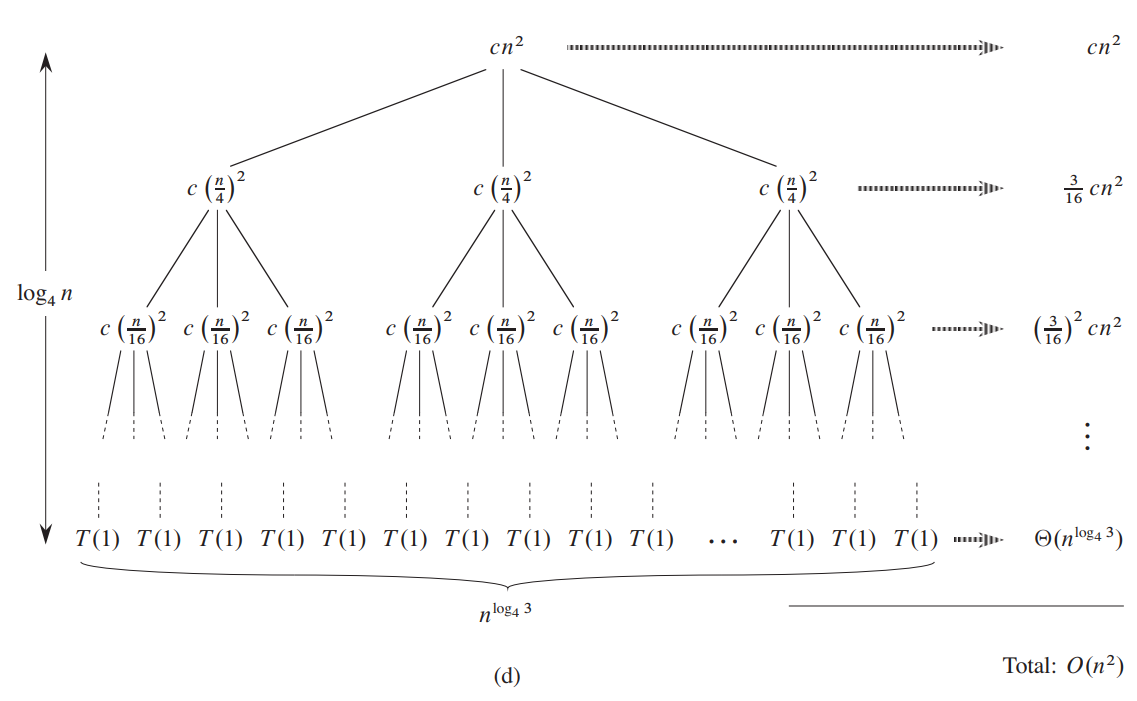
\includegraphics[width = 1\linewidth]{Images/3.png}
\end{center}
\subsubsection{Metodo dell'esperto}
Il metodo dell'esperto permette di risolvere le ricorrenze della forma:
$$T(n) = aT(\frac{n}{b}) + f(n)$$
dove $a \geq 1, b >1$ sono costanti e $f(n)$ è una funzione \textbf{asintoticamente positiva}.
Il metodo dell'esperto dipende dal seguente teorema:
\begin{Teorema}[Teorema dell'esperto]
    Date le costanti $a \geq 1, b > 1$ e la funzione $f(n)$, sia $T(n)$ una funzione definita sugli interi non negativi dalla ricorrenza
    $$T(n) = aT(\frac{n}{b}) + f(n)$$
    dove $\frac{n}{b}$ rappresenta $\floor{\frac{n}{b}}$ o $\ceil{\frac{n}{b}}$. Allora $T(n)$ può essere asintoticamente limitata nei seguenti modi:
    \begin{enumerate}
        \item Se $f(n) = \mathcal{O}(n^{\log_b{a - \varepsilon}})$ per qualche costante $\varepsilon > 0$, allora $T(n) = \Theta(n^{lob_b{a}})$
        \item Se $f(n) = \Theta(n^{\log_b{a}})$ allora $T(n) = \Theta(n^{\log_b{a}} \log{n})$
        \item Se $f(n) = \Omega(n^{log_b{a} + \varepsilon})$ per qualche costante $\varepsilon > 0$ e se $f(\frac{n}{b}) \leq c f(n)$ per qualche costante $c < 1$ e per ogni
        $n$ sufficientemente grande, allora $T(n) = \Theta(f(n))$
    \end{enumerate}
\end{Teorema}
Questo metodo si utilizza principalmente per risolvere le ricorrenze che descrivono i tempi di calcolo degli algoritmi
\textbf{dividi-et-impera}
\section{Programmazione dinamica}
La programmazione dinamica risolve i problemi combinando le soluzioni dei sotto-problemi.
La tecnica dividi-et-impera, divide il problema in sotto-problemi \textbf{indipendenti}, li risolve in modo ricorsivo e, poi, combina
le loro soluzioni per risolvere il problema originale. La programmazione dinamica, invece, può essere applicata quando \textbf{i sotto-problemi non sono indipendenti},
ovvero quando i sotto-problemi hanno \textbf{in comune dei sotto-problemi}. In questo contesto, un algoritmo dividi-et-impera \textbf{svolge molto più lavoro del necessario},
risolvendo \textbf{ripetutamente i sotto-problemi comuni}. Un algoritmo di programmazione dinamica invece \textbf{calcola una sola volta i risultati dei sotto-problemi} e li
salva in una tabella, evitando quindi di ricalcolarli ogni volta che essi si presentano. La programmazione dinamica tendenzialmente si applica ai \textbf{problemi di ottimizzazione}.
Per questi problemi ci possono essere molte soluzioni possibili; quindi si vuole trovare una soluzione con \textbf{valore ottimo} (minimo o massimo). Precisiamo che abbiamo detto \textbf{UNA} soluzione
ottima e non \textbf{LA} soluzione ottima poiché ci possono essere più soluzioni che raggiungono il valore ottimo.
Il processo di sviluppo di un algoritmo di programmazione dinamica può essere suddiviso in una sequenza di quattro fasi:
\begin{enumerate}
    \item Caratterizzare la struttura di una soluzione ottima
    \item Definire in modo ricorsivo il valore di una soluzione ottima
    \item Calcolare il valore di una soluzione ottima, di solito con uno schema bottom-up (dal basso verso l'alto)
    \item Costruire una soluzione ottima dalle informazione calcolate (algoritmo di \textbf{ricostruzione})
\end{enumerate}
Durante la fase 4 possiamo memorizzare anche \textbf{informazioni aggiuntive} utili a semplificare il processo di ricostruzione.
Facciamo un esempio: consideriamo un algoritmo ricorsivo che dia in output l'n-esimo numero di fibonacci: \newline
\begin{algorithm}[H]
\caption{Algoritmo ricorsivo che calcola l'n-esimo numero di fibonacci}
\DontPrintSemicolon
\SetKwFunction{FFibRic}{Fib-Ric}
\Proc{\FFibRic{n}} {
    \eIf{n $\leq$ 1} {
        \Return 1
    } {
        \Return Fib-Ric(n-1) + Fib-Ric(n-2)
    }
}
\end{algorithm}
\noindent
La sua equazione di ricorrenza è:
$$T(n) = T(n-1) + T(n-2) + 2$$
Se provassi a sviluppare la ricorrenza, finirei in un \textbf{loop infinito}. 
Proviamo quindi il metodo dell'albero di ricorsione; supponiamo $n = 5$:
\begin{center}
    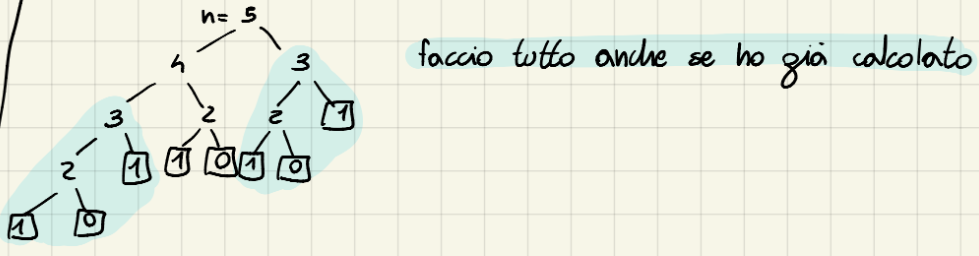
\includegraphics[width = 1\linewidth]{Images/4.png}
\end{center}
notiamo quindi che l'algoritmo \textbf{non si accorge che alcuni calcoli si ripetono}. Notiamo quindi
che l'equazione di ricorrenza è una \textbf{ricorrenza lineare non omogenea}; consideriamo quindi l'equazione
di ricorrenza omogenea associata:
$$T(n) = T(n-1) + T(n-2)$$
supponiamo che $r^n$ è una soluzione:
$$r^n = r^{n-1} + r^{n-2}$$
moltiplichiamo entrambi i lati per $r^2$ e otteniamo:
$$r^2 \cdot r^n = r \cdot r^n + r^n$$
dividiamo entrambi i lati per $r^n$ e otteniamo:
$$r^2 = r + 1 \Rightarrow r^2 - r - 1 = 0$$
il quale è anche il polinomio caratteristico della ricorrenza. Il discriminante di questa equazione di secondo grado è $\Delta = 5$, quindi le due radici del polinomio sono:
$$r_{1,2} = \frac{1 \pm \sqrt{5}}{2}$$
notiamo quindi che la supposizione $T(n) = r^n$ è vera! Poiché $r_1 \neq r_2$ allora l'equazione di ricorrenza omogenea associata diventa:
$$T(n) = c_1 \left (\frac{1 + \sqrt{5}}{2} \right )^n + c_2 \left (\frac{1 - \sqrt{5}}{2} \right )^n$$
per risolvere la ricorrenza, dobbiamo aggiungere una soluzione particolare alla soluzione generale dell'equazione di ricorrenza omogenea associata (Proposizione 1.2.2), cioè quindi dobbiamo
trovare un certo $k$ tale che:
$$T(n) = c_1 \left (\frac{1 + \sqrt{5}}{2} \right )^n + c_2 \left (\frac{1 - \sqrt{5}}{2} \right )^n + k$$
notiamo che la parte non omogenea $f(n)$ della ricorrenza iniziale è costante, quindi dal Corollario 1.2.1 sappiamo che una soluzione particolare
della ricorrenza è \textbf{costante}, in particolare essa è $-2$. Quindi
$$T(n) = c_1 \left (\frac{1 + \sqrt{5}}{2} \right)^n + c_2 \left (\frac{1 - \sqrt{5}}{2} \right )^n - 2 = \Theta\left ( \left (\frac{1 + \sqrt{5}}{2} \right )^n \right )$$
come possiamo riscrivere iterativamente l'algoritmo? \newline
\begin{algorithm}[H]
    \caption{Algoritmo iterativo che calcola l'n-esimo numero di fibonacci}
    \DontPrintSemicolon
    \SetKwFunction{FFibIt}{Fib-It}
    \Proc{\FFibIt{n}} {
        Sia F[0,...,n] un array\;
        F[0] := 1\;
        F[1] := 1\;
        \For{$i \gets 2$ \KwTo n} {
            F[i] := F[i-1] + F[i-2]\;
        }
        \Return F[n]
    }
\end{algorithm}
\noindent
Il tempo di calcolo di questo algoritmo è $T(n) = \Theta(n)$, tuttavia viene "sprecato" dello spazio in memoria per \textbf{memorizzare l'array}.
Notiamo che l'istruzione all'interno del for \textbf{è praticamente uguale alla relazione di ricorrenza presentata in precedenza}; la programmazione dinamica
è quindi \textbf{strettamente legata alla ricorsione} e a come essa \textbf{definisce la STRUTTURA della soluzione}.
\subsection{LCS - Longest Common Subsequence}






\end{document}
